\documentclass{article}

\begin{document}

\setlength{\parindent}{6ex}

\indent

Before introducing YOLO9000, one has to explain YOLOv2 since YOLOv2 is the 
improved version of YOLO in detection performance and speed while keeping 
the real-time speed of detection. YOLO9000 refers to a joint training method on 
object detection and classification. Using this joint training method, one can 
detect objects that do not have any labelled detection data. Now, YOLOv2 will be 
explained and later, YOLO9000 will be explained. \par

As the name of the article suggested, YOLOv2 will be explained in three 
different perspectives: Better, faster, stronger \cite{yolo9000cite}. While better and faster 
refer to a performance increase of YOLO which is YOLOv2, stronger refers to 
YOLO9000. 

\begin{enumerate}
    \item Better
    \begin{itemize}
        \item Analyzing the sufferings of YOLO, one can see that YOLO suffers from 
        localization and having a low recall rate. Thus, the aim is to improve 
        recall and localization while maintaining classification accuracy.
    \end{itemize}
    \begin{enumerate}
        \item Batch Normalization
        \begin{itemize}
            \item Applying batch normalization leads to significant improvement in 
            performance and also it reduces the need for other forms of 
            regularizations. One can remove dropout from the model without 
            overfitting.
            \item Batch normalization leads to a 2\% increase in mAP.
        \end{itemize}
        \item High-Resolution Classifier
        \begin{itemize}
            \item Training of YOLO occurs in two phases: first, convolutional 
            layers are trained on ImageNet classification task on image resolution 
            of 224 x 224. Then, the convolutional layers are trained for detection 
            on image resolution of 448 x 448. This causes the detector to switch itself 
            for learning detection for new resolution simultaneously.
            \item In YOLOv2, before the detector is switched for learning detection, 
            the classifier network is trained for 448 x 448 resolution images for 10 
            epochs on ImageNet. Thus, a time is provided for the network to adjust 
            itself to work better on high resolution.
            \item High-Resolution Classifier leads to a 4\% increase in mAP.
        \end{itemize}
        \item Convolutional with Anchor Boxes
        \begin{itemize}
            \item The Fully-connected layers in the architecture of YOLO are removed 
        and instead of fully-connected layers, anchor boxes are used to predict 
        bounding boxes. Input resolution is decreased from 448x448 to 416x416
        to have a single center feature map: 13x13 feature map. In YOLO, 
        predictions are made with 98 bounding boxes, however, in YOLOv2, 
        predictions are made with more than a thousand bounding boxes.
        Thus, the mean average precision is decreased from 69.5 to 69.2 but 
        the recall is increased from 81\% to 88\%. This tradeoff is worth to do.
            \item There are two issues using anchor boxes with YOLO. The first 
        one is that box dimensions are hand picked which can lead the network 
        to learn hard. If initialization may be done better, the network can learn 
        better. The other one is model instability especially in early iterations 
        of training. Unconstrained anchor boxes can cause a box to appear anywhere 
        in the given image.
        \end{itemize}
        \item Dimension Cluster
        \begin{itemize}
            \item The dimension cluster is developed to handle hand-picked dimensions
        of anchor boxes. To find good anchor boxes for the network, k-means clustering is run 
        over training set bounding boxes. 
        \end{itemize}
        \item Direct Location Prediction
        \begin{itemize}
            \item Direct Location Prediction is developed to handle model instability. 
        The anchor boxes are constrained as bounding boxes in YOLO. Thus, predictions 
        are made relative to the location of the grid cell each anchor boxes belong. This 
        bounds the predicted values 0 and 1. Also, using offsets from the top-left of the image, the 
        correct and constrained locations can be found. 
            \item Using dimension cluster with direct location prediction leads to a 5\% increase 
        over the version with anchor boxes.
        \end{itemize}
        \item Fine-grained Features
        \begin{itemize}
            \item As mentioned above, YOLOv2 predicts with 13x13 feature maps. While this is 
        enough for large objects, it may perform worse in small objects. To handle this problem, 
        a passthrough layer is connected from a 26x26 feature map to a 13x13 feature map. 
        By reshaping 26x26 map to 13x13 map and concatenating them leads to 1\% performance increase. 
        \end{itemize}
        \item Multi-scale Training
        \begin{itemize}
            \item Multi-scale training aims to make the detector more robust 
            to running images of different sizes. Thus, the detector chooses a new 
            image dimension size in every 10 epochs during training from a list of 
            sizes \{320, 352, ...., 608\}.
            \item There is a tradeoff between speed and accuracy since the detector 
            performs faster when image size is smaller but accuracy is worse when 
            image size is smaller.
        \end{itemize}
    \end{enumerate}
    \item Faster

    The main motivation of YOLO is to design a detector that performs 
    real-time object detection while maintaining the detection accuracy as high 
    as possible. To increase detection performance, some features of the detector 
    have to be more complex but designing a more complex architecture causes 
    slower detection speed. To create space for more complex features, in 
    YOLOv2, speed of the backbone network is increased as follows:
    \begin{itemize}
        \item VGG16 requires 30.69 billion floating-point operations for a single 
        pass over a single image at 224 x 224 resolution \cite{yolo9000cite}.
        \item YOLO framework uses a custom backbone network based on GoogleNet 
        architecture. This network uses 8.52 billion operations, however, it works 
        slightly worse than VGG16.
        \item Thus, in YOLOv2, a new classification model is used as a backbone network 
        which is called DarkNet19. This network requires 5.58 billion of operations.
        \item Their accuracy on ImageNet as follows:
        \begin{enumerate}
            \item VGG16: 90.0\% top-5 accuracy.
            \item YOLO: 88\% top-5 accuracy.
            \item DarkNet19: 91.2\% top-5 accuracy.
        \end{enumerate}
    \end{itemize}
    \item Stronger
    
    \begin{figure}
        \centering
        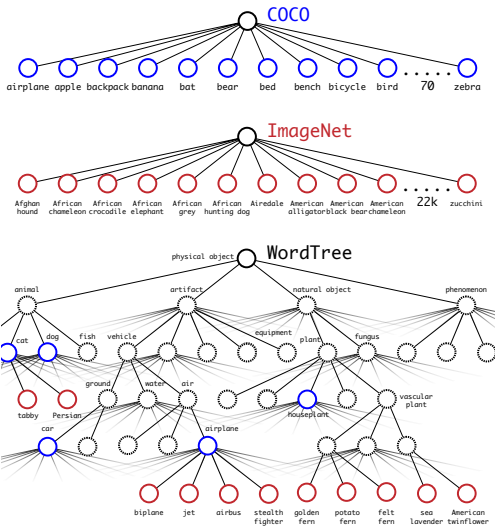
\includegraphics[width=\textwidth]{wordtree}
        \caption{Combining ImageNet and COCO using WordTree hierarchy}
        \label{fig:wordtree1}
    \end{figure}
    
    As mentioned before YOLO9000 is a joint training method on classification and detection 
    data. Detection dataset is used to learn information required to detect such as bounding 
    box coordinate prediction, objectness, etc. Classification dataset is used to expand the 
    number of category detector can detect. During training, detection and classification 
    datasets are used together. When an image is labeled for detection, then, backpropagation 
    can be done overall architecture. Yet, if an image is labeled for classification, then, 
    backpropagation can be done over classification parts of the architecture. The problem in this 
    approach is detection datasets have common labels such as dog, cat, etc but classification 
    datasets have more specific labels such as Norfolk terrier, Yorkshire terrier, etc. 
    WordNet is used to pull labels. WordNet is a language database that structures and relate 
    concepts. As you can see in figure \ref{fig:wordtree1}, WordTree is used to combine 
    detection (COCO) and classification (ImageNet) datasets. Conditional probabilities are used 
    to predict classifications. An example can be seen in figure \ref{fig:condprob1}.
    
    \begin{figure}
        \centering
        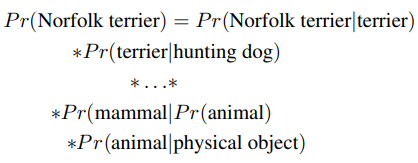
\includegraphics[width=0.75\textwidth]{condprob}
        \caption{Classification calculation example for WordTree}
        \label{fig:condprob1}
    \end{figure}
\end{enumerate}
\end{document}